\section{Evaluation}
\label{sec:evaluation}

In this section, we provide evaluation results for \sysname{}:

\begin{itemize}[itemsep=0pt, topsep=1pt]
\item[\autoref{sec:perf-modeling}] Compared with naive approaches (random and
  gradient-based search), \sysname{} finds a Pareto front that is closer to the
  optimal (\autoref{fig:bo}).
\item[\autoref{sec:runtime}] For all applications, \sysname{} achieves bounded
  service latency across various network conditions (\autoref{fig:end-to-end}).
\end{itemize}

\subsection{Performance Modeling}
\label{sec:perf-modeling}

This section shows that BO can effectively explore the large design space and
come up with a better Pareto-optimal parameter set. We compare \sysname{} with
two baseline profilers: $(i)$ greedy approach as described in
VideoStorm~\cite{zhang2017live}; $(ii)$ random sampling.

Greedy converts MOO into SOO with a parameter $X = \beta$ $A - \beta T$. It
starts with a random configuration $c$ and then picks a neighbor configuration
(by changing the value of a random dimension). If the new configuration $c'$
returns a higher $X$, it updates and iterate form $c'$ again. Otherwise, it
picks a different neighbor $c''$ by changing another dimension. It starts with
three random starting point; it also evaluate a number of random $\beta$.

\autoref{fig:bo} shows that with the same budget (the number of parameters to
evaluate), our profiler can find parameters with better trade-offs between
application accuracy and processing times.

\begin{figure}
  \centering
  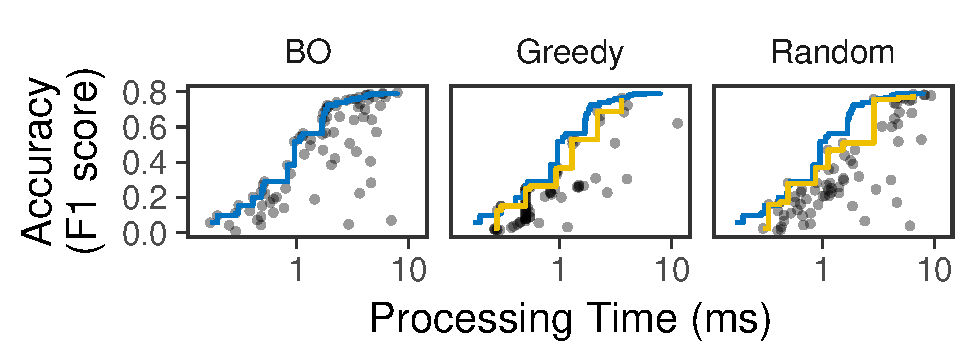
\includegraphics[width=0.95\columnwidth]{figures/profiling.pdf}
  \caption{Using Face as an example, BO evaluates 50 configurations and
    recommends 29 configurations as the Pareto-optimal boundary (the blue
    line). Greedy and Random find sub-optimal Pareto configurations with a
    budget of 80 evaluations (the yellow line in each figure).}
  \label{fig:bo}
\end{figure}

\newpage

\subsection{Runtime Evaluation}
\label{sec:runtime}

To make \sysname{} story compelling, we are convincing the readers the following
points:

\begin{enumerate}[leftmargin=*, itemsep=5pt]
\item Heavy computations are beyond the capabilities of end devices. (Face
  Detection on RPi takes 327 ms). While on a modest workstation, only 27 ms.
\item Naively offloading computation to the cloud does not offers bounded
  response times. Show time series or statistics by injecting traffic or
  additional workload.
\item One can use edge computing, but it is not clear what edge devices are
  capable.
\item To effectively utilizing available resources, cloning can help. Cloning
  without adaptation is not useful on low end devices.
\item Cloning with performance modeling improves.
\item Cloning with performance modeling and server rejection (SLO-awareness)
  improve further.
\end{enumerate}

Point 1, 2, 3 should have been shown in intro and motivation. We only show their
numbers here as reference lines in figures. The runtime experiment is mainly
focusing on demonstrating point 4/5/6, that is, how effective are differential
redundancy and server triage.

\textbf{Methodology:} RPi as the end device, modest server as edge (with and
without GPU), and Amazon EC2 as server (with GPU). RPi and the edge exist within
the same network (~1-2 ms latency).

\begin{figure}
  \centering
  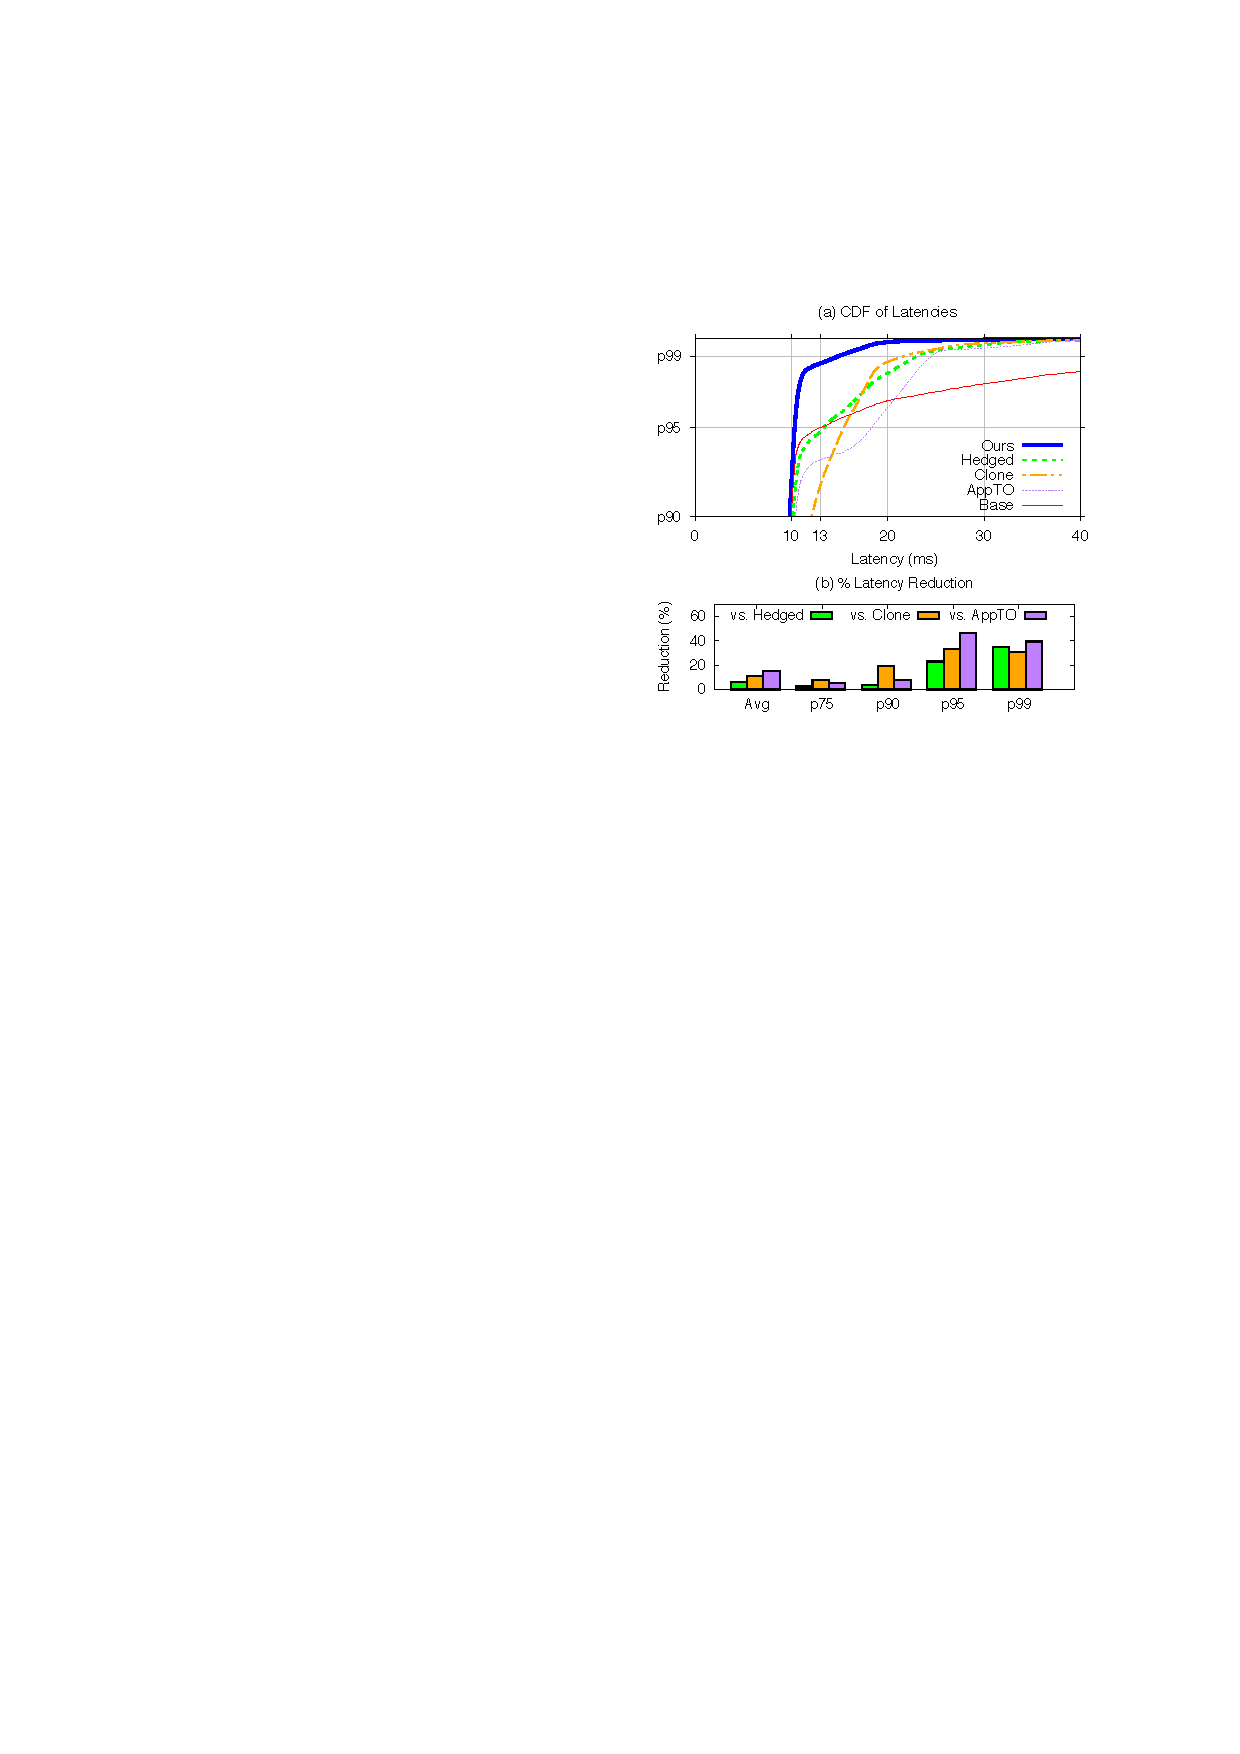
\includegraphics[width=0.95\columnwidth]{figures/runtime-mock.pdf}
  \caption{Compared with other techniques used in reducing tail latency,
    \sysname{} is able to maintain a lower latency bound.}
  \label{fig:eval-runtime}
\end{figure}

\begin{figure}
  \centering
  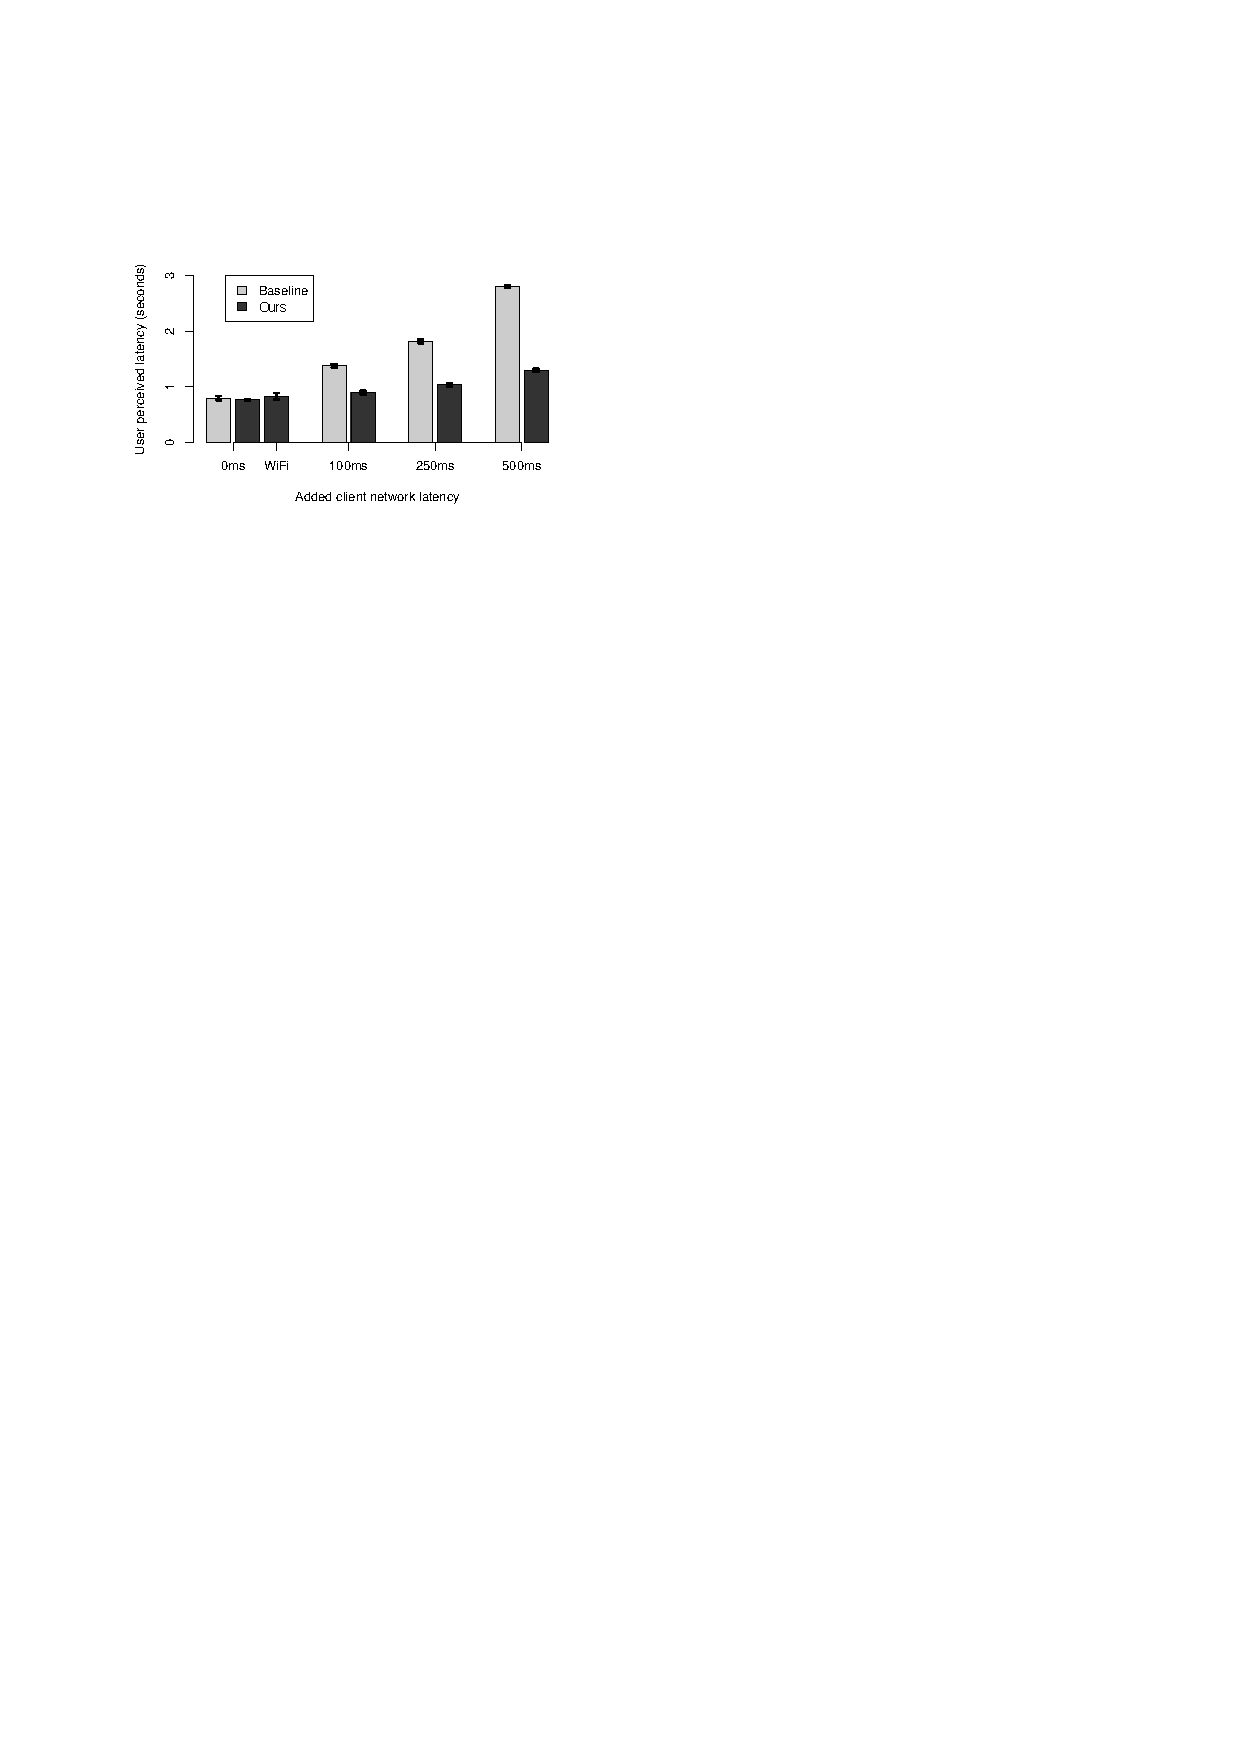
\includegraphics[width=0.95\columnwidth]{figures/eval-net-conditions.pdf}
  \caption{Under different network conditions, \sysname{} maintains bounded
    response times.}
  \label{fig:end-to-end}
\end{figure}

\newpage

Edge computing promises closer resources to end devices, offering better
response time guarantees. While edge servers can be orders-of-magnitude more
powerful than mobile devices, its capability may be limited by budget. We
evaluate the performance \sysname{} with different capabilities of the edge
(with and without GPU).

\subsection*{Serving Overhead}
\label{sec:serving-overhead}

To evaluate our technique against workload variation, we compare \sysname{} with
TensorFlow Serving (TFS), the state-of-the-art framework for deep
learning. While TFS supports loading and serving multiple models, it is more
designed for multiple versions of the same model (in the scenario of A/B
testing). For our evaluation, we only compare us against TFS with one model. The
evaluation is also limited to Object, because TFS is designed for DL
applications and integrating OpenCV algorithms would take too much time for
little purpose. The goal here is to show that \sysname{} adds little overhead
under normal conditions (performance on par with TFS) and is able to adapt and
maintain SLO during service contention (better tail performance).


\newpage

%%% Local Variables:
%%% mode: latex
%%% TeX-master: "../serving"
%%% End:
